
%\usepackage{color}
%\usepackage{graphicx}
%\usepackage{multirow}
%\usepackage{wrapfig}
%\usepackage[export]{adjustbox}
%\usepackage{caption}
%\usepackage{subcaption}
%\usepackage{float}
%%%%%%%%%%%%%%%%%%%%
% - - - - - - - - PART JOAN - - - - - - - - - 
%%%%%%%%%%%%%%%%%%%%
\section{First Placement}
The aim of this part is to explain the first placement of the constellation. It is divided in two parts, the first one is intended to give a first approach to the logistics involved in the first placement. The second one is focused on the maneuver required so as to deploy the satellites into orbit. 
\subsection{First Placement logistics}
The objective of this section is to give a general idea of the first placement logistics. Although some temporal data is provided, it is a qualitative explanation, only to clarify the order in which the different elements must be purchased, assembled, transported, etc. % Since this section does not attempt to provide neither exact data nor exact procedures
Rocket Lab provides two gantt diagrams on which their launching procedure is explained (images \ref{fig:gantt1} and \ref{fig:gantt2}) 

\begin{figure}[h!]
\centering 
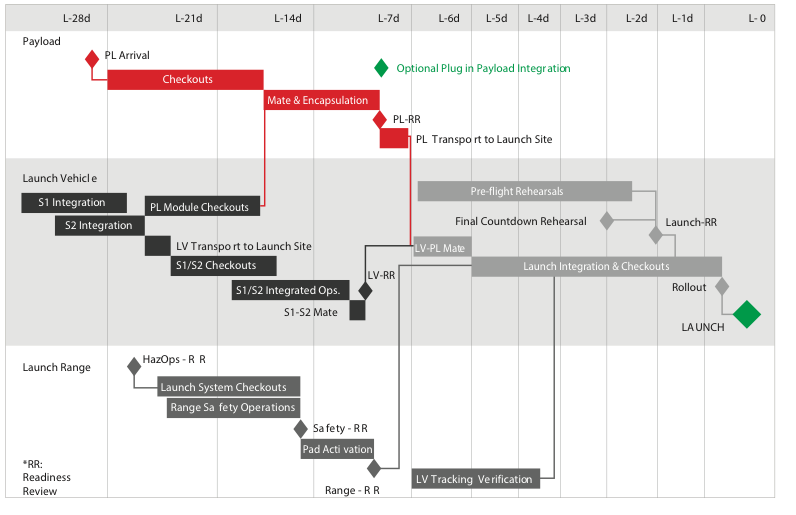
\includegraphics[scale=0.7]{./sections/Constellation_Deployment/S4-First_Placement/Images_S4/Picture_1_S4.png} 
\caption{Launch Range Operations Flow/Schedule}
\label{fig:gantt1}
\end{figure}

\begin{figure}[h!]
\centering 
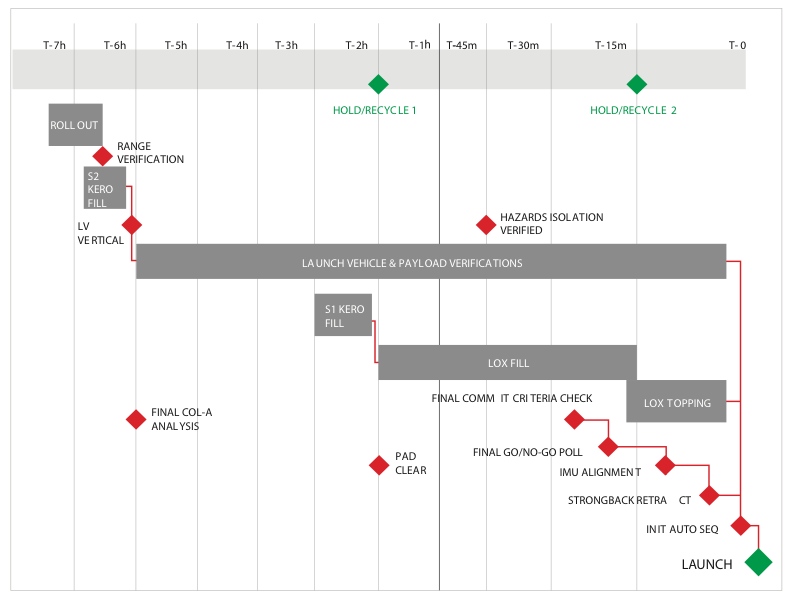
\includegraphics[scale=0.7]{./sections/Constellation_Deployment/S4-First_Placement/Images_S4/Picture_2_S4.png} 
\caption{Countdown Operations Flow}
\label{fig:gantt2}
\end{figure}

%
%\newline
%\begin{figure}{}
%    \centering
%    \begin{subfigure}[!ht]{0.8\textwidth}
%        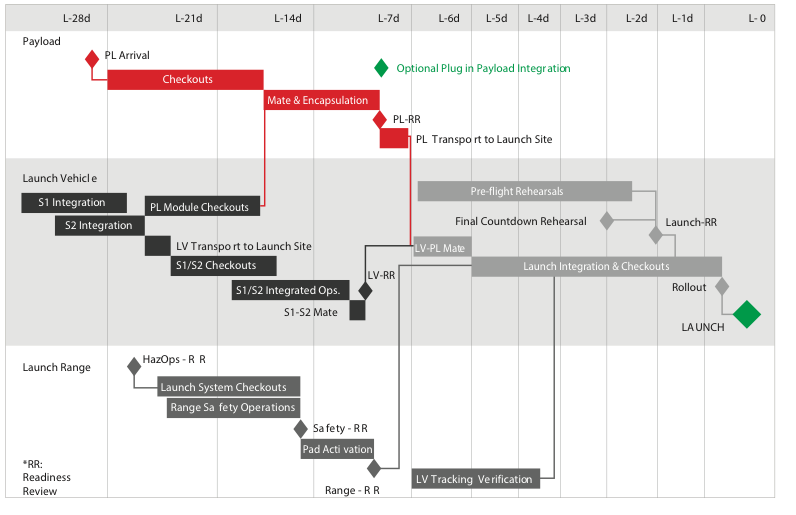
\includegraphics[width=\textwidth]{./sections/Constellation_Deployment/S4-First_Placement/Images_S4/Picture_1_S4.png}
%        \caption{Launch Range Operations Flow/Schedule}
%        \label{fig:gantt1}
%    \end{subfigure}
%    \begin{subfigure}[!ht]{0.8\textwidth}
%        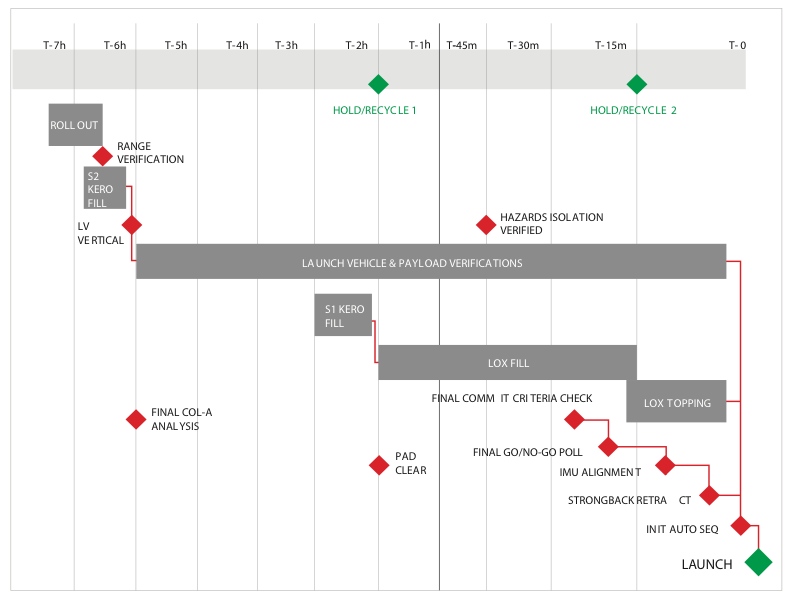
\includegraphics[width=\textwidth]{./sections/Constellation_Deployment/S4-First_Placement/Images_S4/Picture_2_S4.png}
%        \caption{Countdown Operations Flow}
%        \label{fig:gantt2}
%    \end{subfigure}
%    \caption{Launching Logistics RL}\label{fig:animals}
%\end{figure}


The constellation has 168 3U CubeSats distributed in 8 orbital planes. One of the conclusions stated in the Launching System section  is that the quickest way to deploy the whole constellation is by carrying out one launching per orbital plane, consequently, the first placement consists on 8 launchings and all the logistics around them. Rocket Lab is capable of launching once a week, therefore, the first placement takes 8 weeks. Due to the magnitude of the mission, the whole rocket is filled with Astrea satellites, hence, there is no need to share it with other missions. Also, Rocket Lab offers an online booking procedure to reserve a date, however, The Payload User's Guide (provided by Rocket Lab) recommends contacting directly with them in case of filling several rockets with a mission instead of booking online.  
\newline
Since the schedule of Rocket Lab is fixed, the logistics needed in order to deliver the payload on time are going to be explained starting from the launching day, going back in time until the first movements in Terrassa, where the satellites are assembled. 
The launching day is designed L henceforth, and all the other ones are referred to this one (eg. L-30d means 30 days before launching). 


As seen in figure \ref{fig:gantt1}, Rocket Lab needs 28 days to prepare the payload, place it into the rocket and prepare the rocket itself. Thus, the CubeSats have to arrive at the Rocket Lab launching facilities the L-28d. The satellites are assembled in Terrassa, hence, they have to be brought to New Zealand. Due to the large amount of CubeSats, the chosen transport is sea transportation. The estimated time from Terrassa to New Zealand is 30 days, so the CubeSats have to leave Terrassa the L-58d. At this point, there is two options. First, the 168 satellites can be divided in groups of 21 (number of sats in an orbital planes) and sent separately to New Zealand so that every group arrives 28 days before its departure. The other option is to send all 168 CubeSats at the same time so that they arrive 28 days before the first launching. Each option has its pros and its drawbacks. Option one does not need to store the satellites in Rocket Lab facilites, conversely, the logistics of carrying each group of satellites separately is complicated. Option two allows to assemble all the satellites and send them in one ship, however, once they arrive to their destination, they have to be stored somewhere until their departure day arrives. Option two is selected because it is simpler and it is more likely to not cause delays delivering the payload to Rocket Lab, in addition, it is concluded that sending eight ships with one week separation is not as efficient as sending a single one. 
\newline
The estimated time of assembling the satellites is twelve months, consequently, they have to be ordered the L-423d. 
\newline
As clarified above, it is important to remember that the stated times are an approximation and the goal of this section is to give a first idea of the order of the different actions. 
%%%%%%%%%%%%%%%%%%%%%%%%%%%%%%%%%%%%%%%%
% - - - - - - - - - PART ROGER - - - - - - - - - - 
%%%%%%%%%%%%%%%%%%%%%%%%%%%%%%%%%%%%%%%%
\subsection{1st Placement Maneuver}
Once the Constellation is designed, it is essential to plan a proper procedure to put it in orbit. The Constellation is configured in several planes and satellites in each plane which work and communicate together in order to give signal coverage around the globe to finally accomplish their final purpose: intercommunicate other satellites form our customers.
\newline\newline
One of the purposes of the project is to ensure the system is able to provide partial service right from the very beginning of its life, that is since the first orbital plane is put into orbit. Therefore, along with the maneuvers required to separate satellites in a certain orbital plane, the order in which the planes are put into orbit will also be assessed in this section. This particular section is crucial as it describes how the constellation is born.
\subsection{In-Orbit Injection}
It wouldn't be fair to start without mentioning the spaceship that will bring the whole system to life, and this is no more and no less than the Electron, from Rocketlab USA in New Zealand. The Electron is able to carry 24 3U CubeSats at once. Since 21 is the number of satellites needed in 1 orbital plane, it will be able to put one orbital plane into orbit in just one launch using the procedure described in the upcoming paragraphs.
\newline\newline
Before starting any procedure description, it is important to set a start point. The first consideration is that there are still no Astrea satellites orbiting the earth. Therefore it is the first orbital plane that will be put into orbit. It is also considered that the rocket loaded with the 21 satellites has already accomplished all necessary maneuvers after lift-off and has just been able to arrive at the satellite's orbit, that is, proper altitude above Earth and proper tangential velocity. Of course at this point only the 2nd stage of the initial Electron rocket remains. Moreover, this stage is the one responsible of carrying the payload along with every single deployer. Once the start point is set, it is possible to thoroughly describe the procedure.
\newline\newline
At the very described moment the first CubeSat is deployed into its final orbit around the Earth, which is a circular orbit at $542 \,km$ above Earth's surface. In order to deploy the second satellite at a given phase separation from the first one, the rocket must enter into an elliptical orbit with a slower period. Adopting this procedure will allow the needed phase separation between satellites given the fact that after one revolution of the rocket around the Earth, the first satellite will have gone through one revolution and a fraction more. In other words, at the very moment the rocket passes through the initial point which is tangential to the satellite's orbit, the first deployed satellite will be phase-wise ahead of the rocket. Obviously, the elliptical orbit mentioned must be accurately computed in terms of the increments in speed required to enter into it.
\newline\newline
In a more schematic way, the procedure goes as follows:
\begin{enumerate}
\item The rocket goes through the procedure designed by Rocketlab USA to get to the destination orbit. The approximate trajectory during this stage is represented in \ref{orbit1}.Right after entering into the destination orbit, the first satellite is deployed into it as seen in \ref{orbit1} represented with a red dot.
\item Once the latter is completed, the rocket's engine gives it the necessary $\Delta V$ in order to get to the elliptical spacing orbit. In \ref{orbit2} half a revolution of the rocket is represented along with the orbit of the first deployed satellite at the same point in time.
\item After one full revolution of the rocket in the elliptical orbit, the first satellite will have left the right phase spacing with respect to the rocket. At this point the rocket's engine gives the same $\Delta V$ as in 2 but negative. This will cause it to enter again into the circular orbit of the satellites. At this point the rocket deploys the second satellite as shown in \ref{orbit3}. Right after this deployment the rocket enters into the elliptical orbit again.
\item \ref{orbit4} represents again half a revolution of the rocket in the elliptical orbit along with the deployed satellites so far.
\item Finally, the rocket reduces its velocity again to enter into the circular destination orbit in order to deploy the third satellite (\ref{orbit5}).
\item The procedure is iterated until the orbital plane is full.
\newline\newline
\end{enumerate}
\begin{figure}[H]
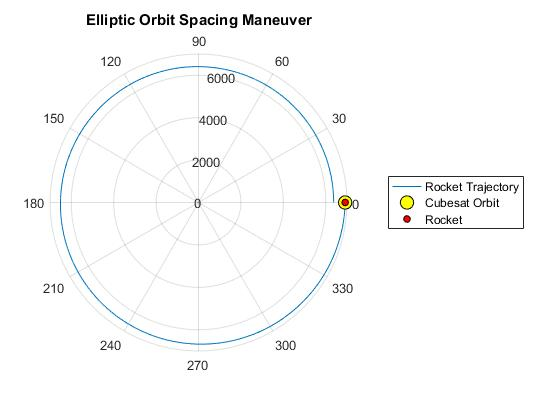
\includegraphics[scale=0.7]{./sections/Constellation_Deployment/S4-First_Placement/Images_S4/Picture_3_S4.jpg}
\caption{Rocket's trajectory from lift-off to final orbit.}
\label{orbit1}
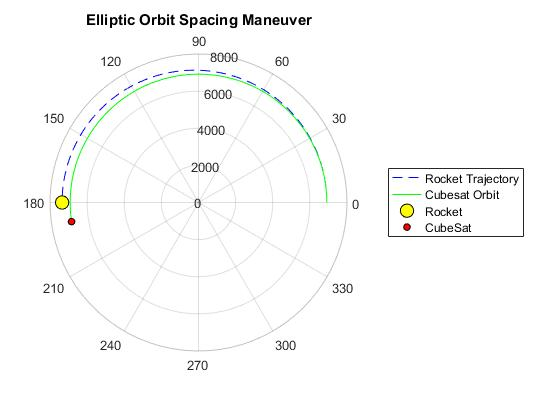
\includegraphics[scale=0.7]{./sections/Constellation_Deployment/S4-First_Placement/Images_S4/Picture_4_S4.jpg}
\caption{Half of a revolution of the rocket in the elliptical spacing orbit.}
\label{orbit2}
\end{figure}
\begin{figure}[H]
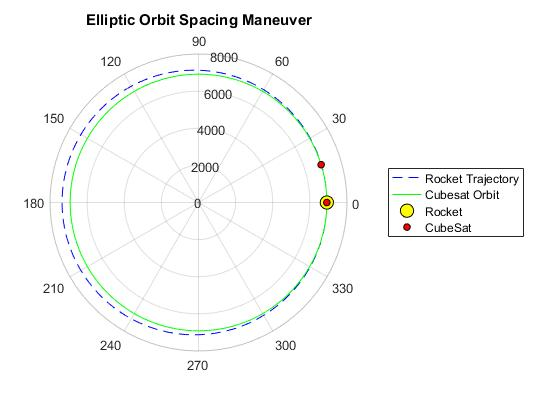
\includegraphics[scale=0.7]{./sections/Constellation_Deployment/S4-First_Placement/Images_S4/Picture_5_S4.jpg}
\caption{Deployment of the second satellite.}
\label{orbit3}
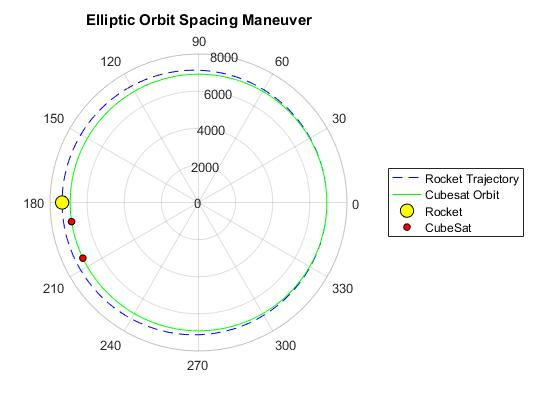
\includegraphics[scale=0.7]{./sections/Constellation_Deployment/S4-First_Placement/Images_S4/Picture_6_S4.jpg}
\caption{Half of a revolution of the rocket after the deployment of the second satellite.}
\label{orbit4}
\end{figure}
\begin{figure}[H]
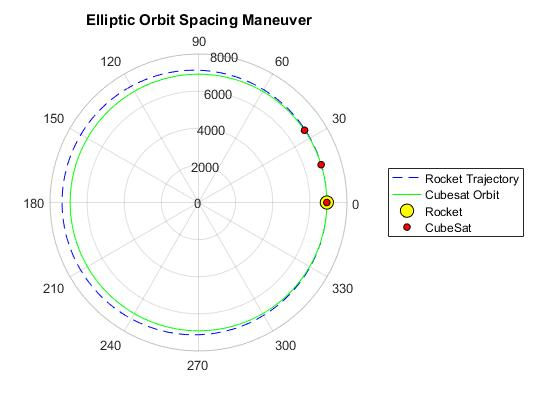
\includegraphics[scale=0.7]{./sections/Constellation_Deployment/S4-First_Placement/Images_S4/Picture_7_S4.jpg}
\caption{Deployment of the third satellite.}
\label{orbit5}
\end{figure}
Having pointed all of the above, it would make no sense to proceed without thoroughly going through the calculations of every single one of the required parameters to perform the manoeuvre. The first thing to take into account is the number of satellites for orbital plane. A number of 21 satellites per plane has been established, thus, a separation of $360^\circ/21 = 17.14^\circ$ between satellites will have to be accomplished. The velocity of the satellites and the period of their orbit is now computed:
\newline
\begin{center}
$V_s = \sqrt{\frac{GM_t}{R_t\,+\,h}} $
\newline\newline
$T_s = \frac{2\pi*(R_t\,+\,h)}{V_s}$\newline
\end{center}
Where $R_t$ and h are Earth's radius and height above Earth's surface respectively. For $h = 542 \,km$, the values obtained are $V_s = 7,589.6 \,m/s$ and $T_s = 5,723.1 \,s$. Let's call the spacing between satellites $\theta = \frac{360^\circ}{21} = 17.14^\circ$ and $R = R_t \,+ \,h$. Using these values it is possible to compute the period of the elliptical orbit, $T_r$, along with the rest of the parameters:
\newline
\begin{center}
$T_r = T_s\,+\,\frac{\theta R}{V_s} = 5,995.6\,s$
\newline\newline
$a = (\frac{T_r}{2\pi}^2GM_t)^\frac{1}{3}=7,130.8\,km$
\newline\newline
$R_1 = R;\;\;\;R_2=2a\,-\,R_1$
\newline\newline
$c = a\,-\,R_1;\;\;\;b = \sqrt{a^2\,-c^2}$
\newline\newline
$\epsilon = \sqrt{1\,-\,\frac{b^2}{a^2}}=0.0305$
\newline\newline
$\Delta V = \sqrt{\frac{GM_t}{R1}}\,(\sqrt{\frac{2R_2}{R1\,+\,R2}}-1)=115.01\,m/s$
\newline\newline
\end{center}
Astrea's main purpose when it comes to 1st placement is to provide service as quickly as possible. This means that the time it takes to put a plane into orbit is crucial. This time will be determined by the period of the elliptical separation orbit that the rocket uses between deployments and of course by the number of satellites in each plane. Since 21 are the satellites that need to be put in orbit, 21 elliptical orbits will be needed. Therefore the time needed for one orbital plane is $3200\,s + 21*T_r = 129,191.6\,s$ which means 35.9 hours.
\subsubsection{Plane Order}
Having described the procedure used to put one orbital plane in orbit, it is now time to describe the order in which all of the 8 planes are put into orbit. The fact that establishes one path or another is the fact that satellites can only communicate with neighbours, that is, one satellite can only communicate with its neighbours from the same plane and the neighbours from the neighbour planes.
\newline\newline
When it comes to the order in which the planes are put into orbit, there are two main ways that come to mind. The first one is putting the planes consecutively into orbit. The second one is to put the planes into orbit leaving space between them for future planes. For example plane number one is put into orbit. The second plane to be put into orbit leaves space for one plane in between them. Then the third leaves space for one plane from the second, and so on. Leaving more space than for one plane could also be an option.
\newline\newline
On the one hand, when using the first way the satellites from each plane could communicate with the ones from their neighbourhood. Therefore the range of communication would start being narrower but as new planes are put into orbit, the range would become wider. For instance, when three planes are already working, a given satellite form a customer could communicate with satellites that are at the other side of the planet in a determined range given by the width of signal that those three orbital planes could cover. When new planes are put into orbit this width becomes bigger up until the full globe is covered. Of course the main drawback of using this consecutive way of putting planes into orbit would be the long time of inactivity right at the beginning when few planes are working.
\newline\newline
On the other hand, when using the second described way, the satellites can't communicate with other satellites from neighbour planes but the time of inactivity for customer's satellites would be less as a gap between planes is left for future ones. Nevertheless, this kind of configuration has a huge drawback and it's that when a satellite communicates with one given plane, this one can only communicate with other satellites that are in the range of signal emission of that given plane. This is due to the fact that as neighbour planes are further apart they can't communicate with each other and therefore the range of communication is affected.
\newline\newline.
Having pointed out all of the advantages and drawbacks of each configuration it is time to choose and it all comes down to Astrea's preferences. The configuration that fulfils these preferences for the most part is the consecutive .It allows the satellites to communicate in a broader range as the constellation grows and progressively conquer the sky.





